We present here images that can be interesting but are not fundamental for the report.
\begin{figure}[h]
    \centering
    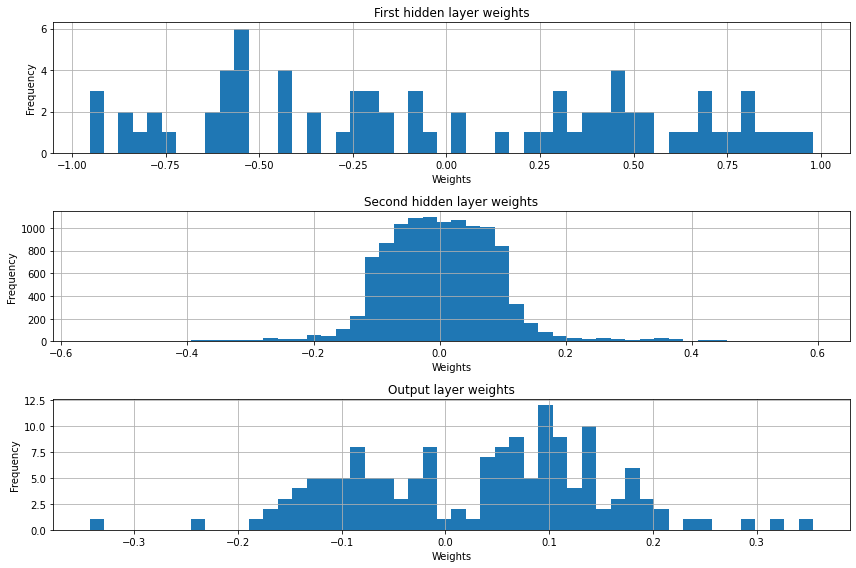
\includegraphics[width=0.8\textwidth]{Images/reg_weights.png}
    \caption{Weight histograms for the different layers of the network.}
    \label{fig:reg_weights}
\end{figure}

\begin{figure}[h]
    \centering
    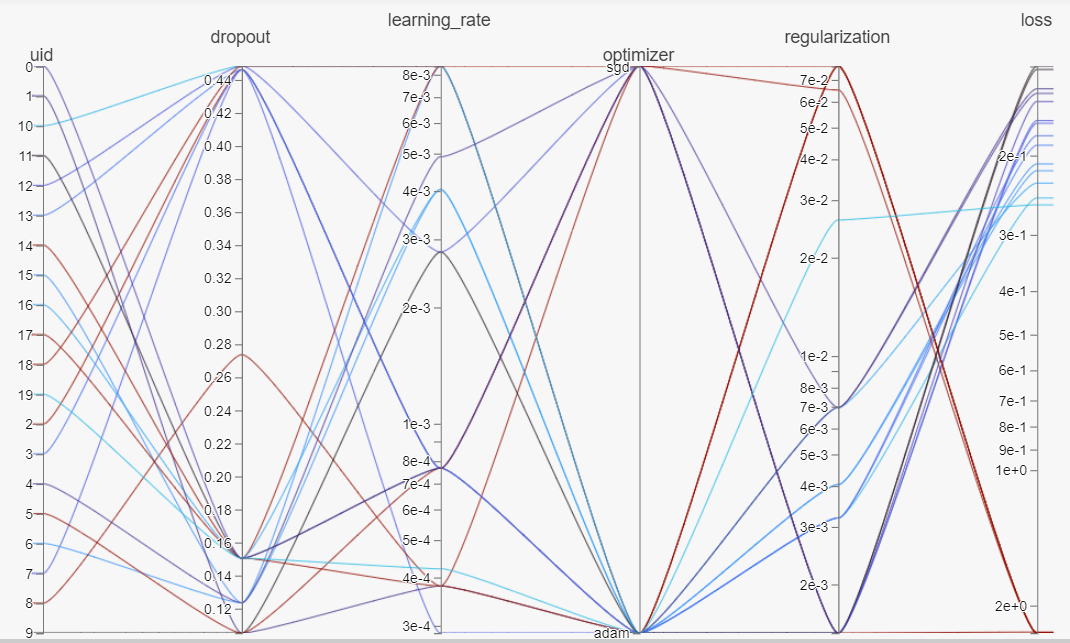
\includegraphics[width=0.8\textwidth]{Images/hyperparams.PNG}
    \caption{Hyperparameters search for the classification task. We plotted with a color which is proportional to the loss function,
    reported in log-scale. The darker the color, the better the result. We notice that a really high L2 regularization 
    usually translates in a low loss score.}
    \label{fig:cl_hp}
\end{figure}